



\section{Architecture of simulation framework} \label{sec:architecture_of_simulation_framework}


The simulation framework described in this section encompasses already described components in Section \ref{sec:r_java_simulation_framework} but enhances the framework by the cloud simulator. The cloud simulator should be able to assess the outcome of different scenarios encompassing data provided by the application server and utilizing forecast models generated on the application server in a previous step. 

The goal was to deliver a complete framework that can handle multiple data sources and is extendable for future work with possibly different data sets and an optional connection to a real cloud environment which could replace the simulated cloud environment that is connected to the framework in this implementation. 

The implementation consists of three parts which will be presented separately below. 

\paragraph{Data management} The first part represents the data handling and management interfaces presented in part already in Section \ref{sec:r_java_simulation_framework}. The purpose of this platform is to have a generic means of parsing and fetching data from various sources that can be defined in advance. For example, data may be fetched from local files that were previously retrieved from energy markets or remote web services that provide energy data of that respective energy market. In addition parsers for different file formats may be defined to automatically parse data and put it into the database for later retrieval. From there arbitrary queries may be executed to retrieve and aggregate data in a specific fashion and execute further tasks based on that data (e.g.~model generation). 

\paragraph{Forecast generation}
The second part consists of a collection of statistical methods that should assist in making accurate forecasts based on the previously collected data. A large scale evaluation of forecast methods has been presented in Section \ref{sec:forecast_model_evaluation} to determine the best forecast models for data from various energy markets. 
The purpose behind these statistical examinations is to provide meaningful and accurate forecasting models that can be utilized by the simulation framework. Eventually the performance of forecasts within the simulation should be examined and compared with approaches based solely on currently available data. It is expected that the application of accurate forecasts to energy price time series within the simulation improves overall performance and thus leads to a reduction in total energy costs. 

\paragraph{Cloud simulation}
The third part constitutes the actual cloud simulation which is based on a previously existing and sophisticated cloud simulator written in Python that incorporates cost models for energy and cooling expenses and is easily extendable by integrating custom schedulers \cite{lucanin2015philharmonic}. In this work custom settings have been applied to allow for a simulation that meets the needs of the framework to integrate different scenarios. Various parts of the simulator needed to be extended and a completely new scheduler has been built to schedule both cost aware and non-cost aware scenarios. It works together well with other parts of the framework s.t.~data can be retrieved from interfaces of the application server and integrated into the cloud simulation. The components are decoupled such that each of them may be replaced by other components easily provided that the same interface is used. 


\subsection{Architectural outline}

The architectural outline provides an overview of all components involved in the presented simulation framework and how they work together. All components may interact with one another via defined interfaces s.t.~either component may be replaced by a similar component with possibly different implementation details but same interfaces. 

\begin{figure}[htbp]
	\centering
	\vspace{-0.4in}
		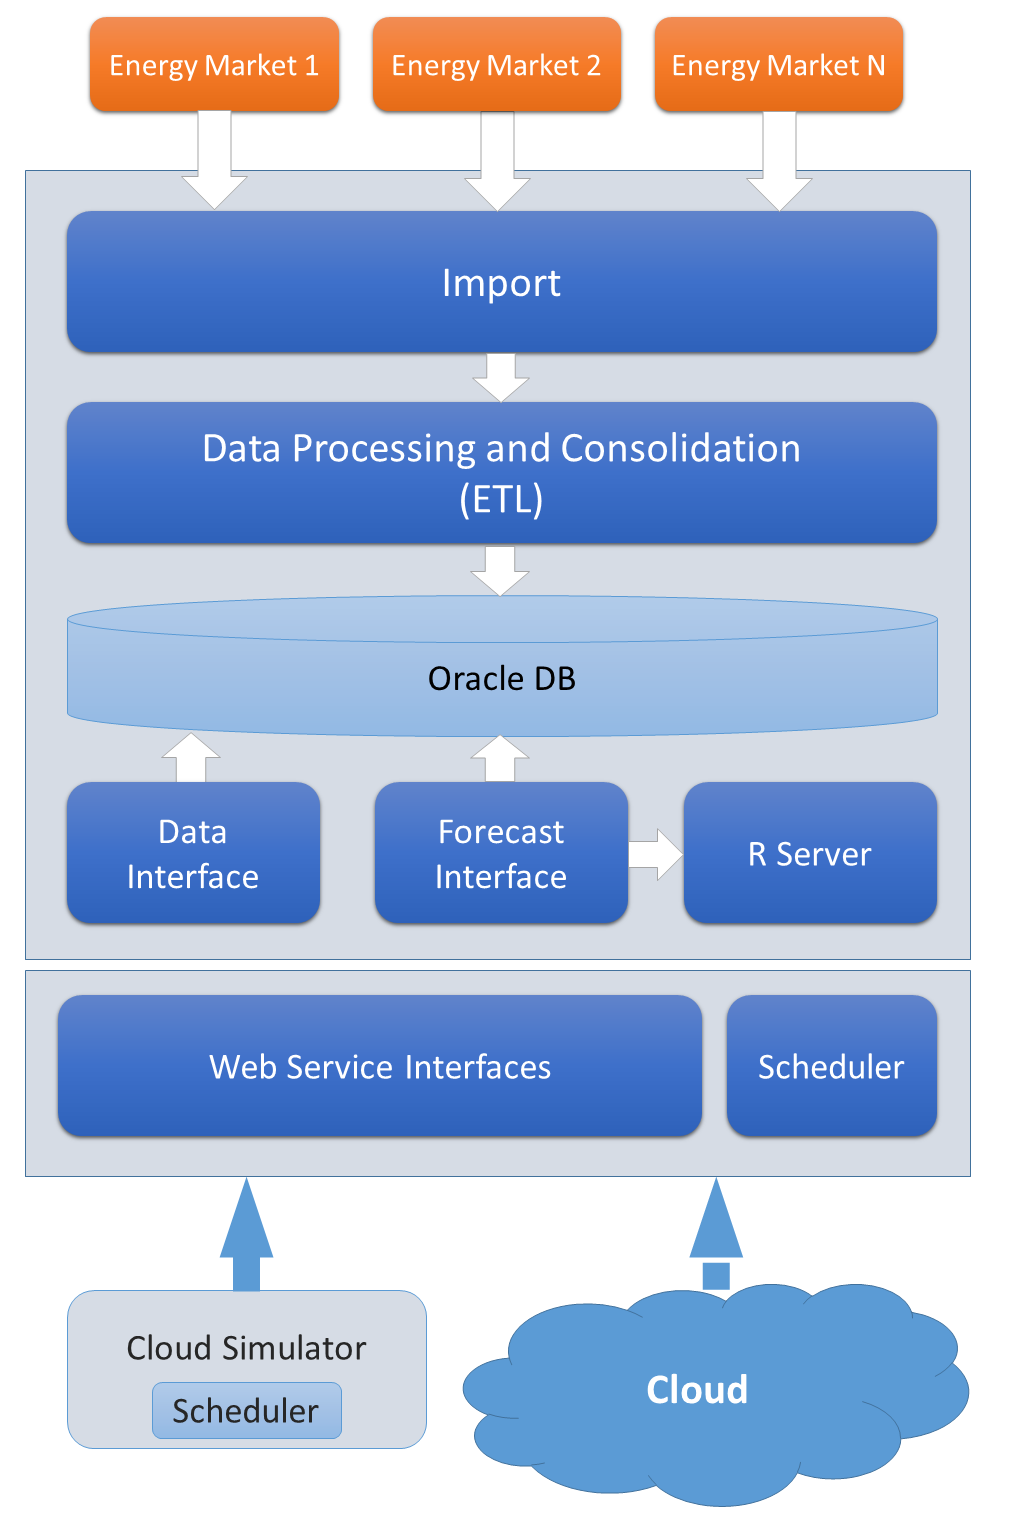
\includegraphics[width=0.5\textwidth]{figures/simulation_framework/Block_Diagram_Architecture.png}
	\caption{Architecture Block Diagram}
	\label{fig:Block_Diagram_Architecture}
\end{figure}

Figure \ref{fig:Block_Diagram_Architecture} depicts a block diagram of the simulation framework that shows which components are included and how they interact with one another. Data retrieval from the energy markets is done by the \textit{Import} module as the first action in the process. Several energy markets and their interfaces may be registered beforehand to retrieve data from these interfaces. 

From the \textit{Import} module the retrieved data is handed over to the \textit{Data Processing and Consolidation} module which transforms the data to a common format such that it can be fed to the database. This process is similar to the well known ETL process (Extract Transform Load)\cite{vassiliadis2002conceptual} which extracts data from various sources, transforms it into a defined data format and loads it into a data warehouse or database. The applied process in this work is similar as parsers for different file formats may be defined that can be configured to parse data from different sources. After the data transformation process the retrieved energy prices are stored in the database from where they may be retrieved for simulation purposes. 

The \textit{Data Interface} contains all methods for data retrieval of prices stored in the database. Thus data is provided to web service interfaces for arbitrary time periods and both day ahead and real time prices. In addition it is possible to query for local or DST corrected bidding dates or retrieving data adjusted to a predefined currency (e.g.~dollars). 

The \textit{Forecast Interface} handles all requests related to model generation and forecasting which is provided by the \textit{R server}. It contains methods defined for large scale forecast evaluation, automated model generation and calculating forecasts for generated models. 

The \textit{R server} does not directly connect to the database but retrieves energy data from the \textit{Forecast Interface} which triggers the generation of forecasting models. The interface used to communicate from Java to R (and vice versa) is called \textit{rJava} \cite{rforge2007rjava} which provides a wrapper to directly execute R code in Java. 

The \textit{Scheduler} may be configured to trigger data import from specific energy markets at a defined time interval (e.g.~every hour or once per day). In this process it may also trigger the generation of forecasting models as the model generation process can take a considerable amount of time depending on the amount of training data provided to the model.

Finally the \textit{Web Service Interfaces} are a means of providing data to external components such as the simulator or a real cloud. 
These interfaces provide data retrieval and forecast interfaces as described previously. They can be used to get historical data from different energy markets and locations as well as time periods for the purpose of getting customized data for simulations. In addition they provide a convenient way of retrieving forecast data for specific locations and periods of time. As soon as forecasting models have been generated for a specific period of time forecasts can be provided instantly for that period. 



\subsection{Components and Interfaces}

In this section a more detailed view on the various components of the framework is provided and the interfaces that exist between them. Figure \ref{fig:Component_Diagram} shows this view in form of a component diagram. 

\begin{figure}[htbp]
	% used to position the image at the horizontal center of the page
	\hspace*{-0.8in}
		% include the graphic rotated by a 90 degree angle and scale to paperwidth and height
		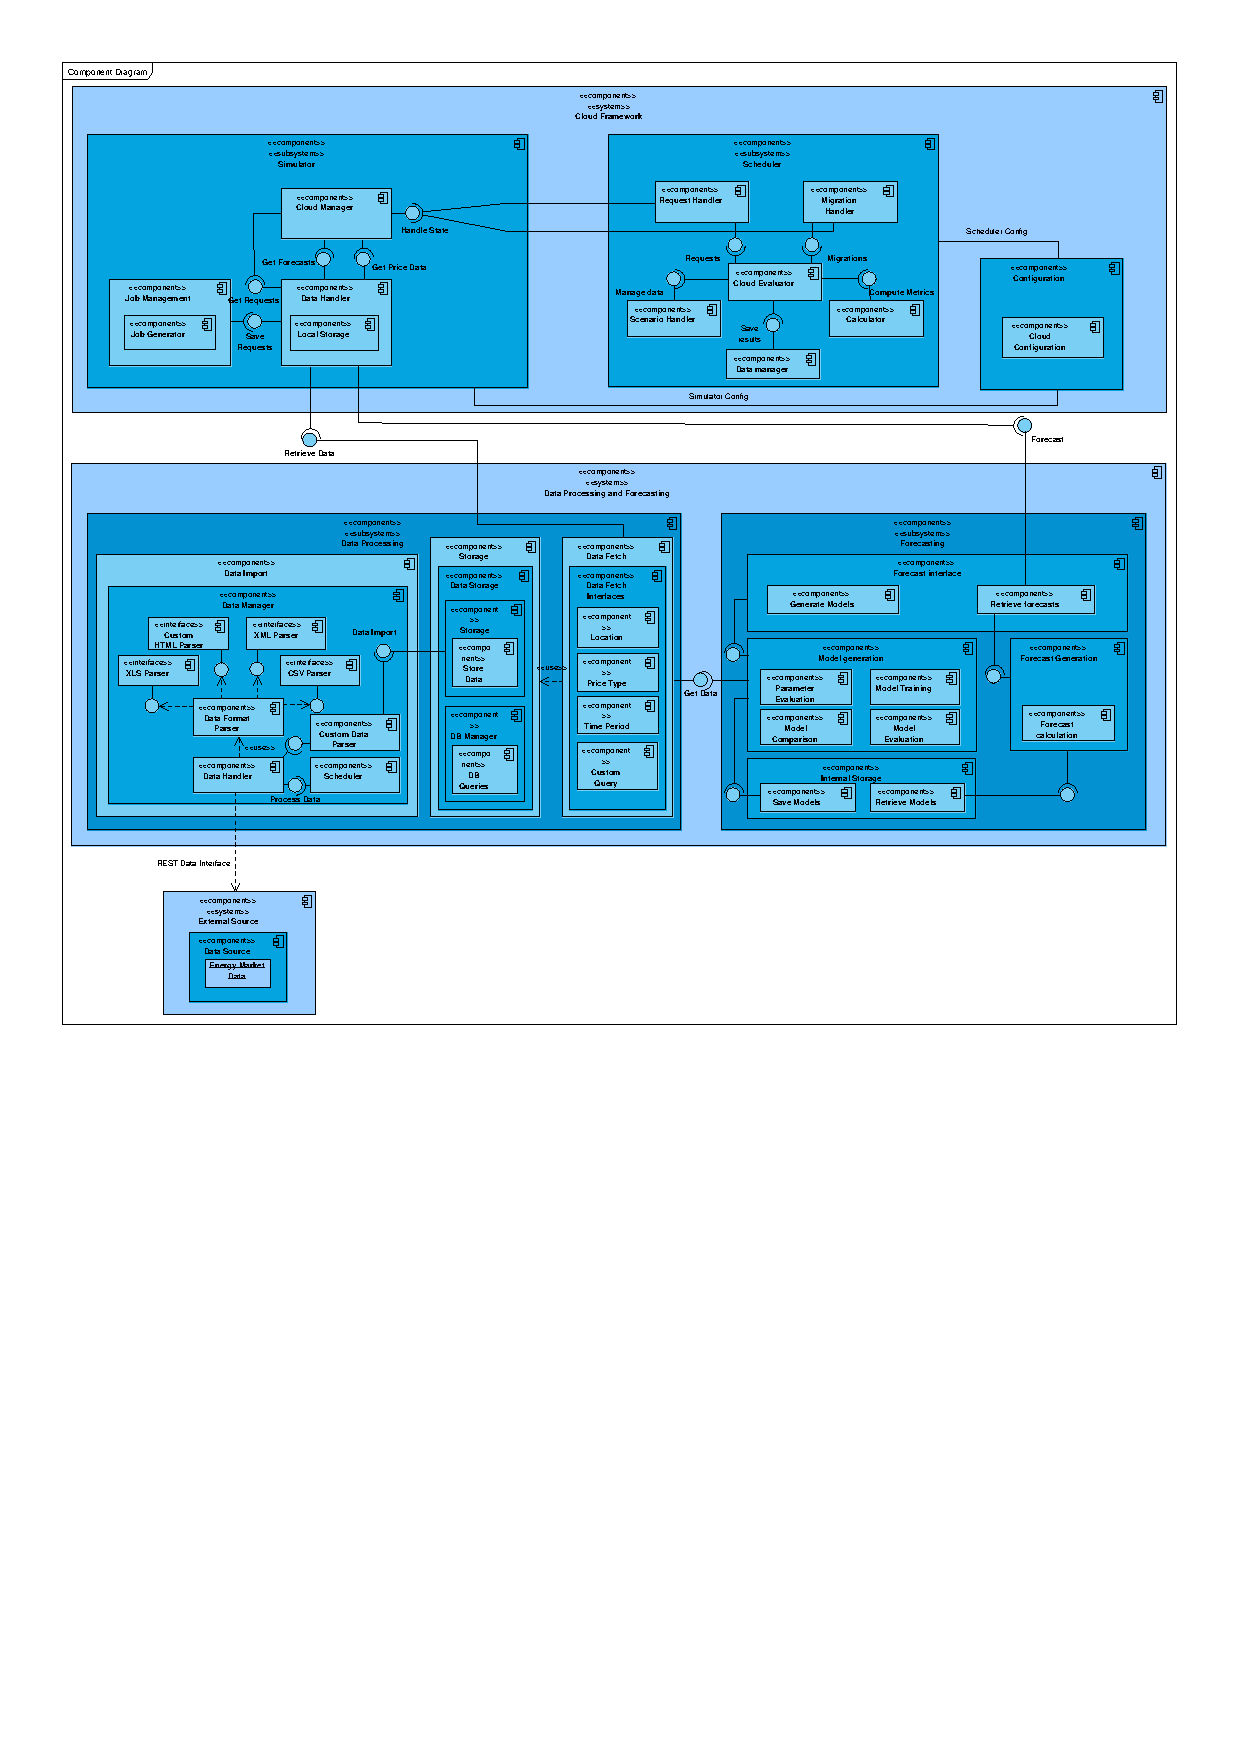
\includegraphics[angle=90,width=\paperheight,height=\paperwidth,keepaspectratio=true]{figures/simulation_framework/Component_Diagram.pdf}
	\caption{Component Diagram}
	\label{fig:Component_Diagram}
\end{figure}

The diagram basically consists of two parts, the \textit{Cloud Framework} and \textit{Data Processing and Forecasting} components. The Cloud Framework contains the \textit{Simulator} and \textit{Scheduler} and is implemented in python \cite{lucanin2015philharmonic}. It is responsible for the actual simulation and application of scheduling algorithms. The Data Processing and Forecasting part consists of the \textit{Data Processing} and \textit{Forecasting} components and is implemented on the Java application server. This component is responsible for data management and forecast operations.

\textit{Data Processing} consists of \textit{Data Import}, \textit{Storage} and \textit{Data Fetch} components. 

The \textit{Data Import} component is responsible to retrieve data from previously registered energy markets as indicated by the dashed line connection to the external data source. The data import can as well be triggered by the scheduler which calls the respective services at the Data Handler. The Data Handler uses appropriate parsers to extract data into a common processable format. When the processing of data is finished the 
data is fed to a \textit{Custom Data Parser} which handles peculiarities such as DST time changes and missing energy price data. The cleared data is then handed on to the Storage component which saves the data to the database. 

The \textit{DB Manager} in the Storage component provides methods for data retrieval which is used by the \textit{Data Fetch} component. 
Different interfaces are provided for executing queries of stored energy price data, e.g.~by location, price type or custom queries. This can in turn be used by the simulator to retrieve energy price data. 

The \textit{Forecasting} component provides interfaces to \textit{Generate Models} and \textit{Retrieve Forecasts}. 

The \textit{Generate Models} component refers to the \textit{Model Generation} component with \textit{Parameter Evaluation}, \textit{Model Training}, \textit{Model Evaluation} and \textit{Model Comparison}. Before model generation it refers to the Data Fetch component for retrieval of energy price data of the desired time period. After the model(s) have been generated they are saved to the \textit{Internal Storage}, i.e.~in the file system of the application server. 

For retrieving forecasts the \textit{Retrieve Forecasts} interface is queried which in turn calls the \textit{Forecast Generation} component. Thus forecasts may be retrieved from models which have been generated and stored previously within the Internal Storage component. 

fetches data from the database and does some data preprocessing that is used for forecasting. After the data has been processed and formatted appropriately it is ready to be analyzed by statistical methods to determine which forecasting model suits best for the selected time series. Different models are trained and compared and the best model is chosen. It is then selected by the Forecast Module and the actual forecasts are calculated which can be queried via a provided public interface that is exposed to external systems. 

The \textit{Cloud Framework} uses the historical price data provided by the \textit{Data Fetch} component to run simulations for various scenarios. It is read into a local storage by a \textit{Data Handler} for further processing of the price data in simulations. In addition, forecasts may be retrieved by the Data Handler at this stage to prevent having an open connection to the application server during simulations. Job requests are generated by the \textit{Job Management} component which reflect certain characteristics or requirements of tasks that should be processed by the Cloud Framework. Requests and energy prices are read by the \textit{Cloud Manager} that keeps track of the cloud's current state. The state is retrieved and modified by the scheduler which retrieves data from \textit{Request} and \textit{Migration Handlers} which is then fed to the \textit{Cloud Evaluator}. The evaluator decides on needs for migrations depending on the given scenario defined by the \textit{Scenario Handler}. It uses a \textit{Calculator} component to compute metrics such as migration energy and VM downtime. 

At each step the Cloud Evaluator gets current request and migration demands and checks metrics for VM migration. If it retrieves a positive result the resources are moved to the respective server. Results are handled by a Data Manager component after the simulation finishes. Both scheduler and simulator components are configurable by a config file defined by the \textit{Cloud Configuration} component. Thus new configuration options are easily added and can be changed at any time to adjust the output of simulations. 




\section{Modeling migration energy} \label{sec:modeling_migration_energy}

Besides the structural outline presented in the previous section important methodologies used by the cloud simulator and scheduler are investigated in detail in the following sections. 

Since the goal of the simulation presented in this work is to reduce energy costs by intelligently migrating resources across geo-distributed data centers an important metric to consider is the migration energy and migration costs. An outstanding paper on this topic has been presented in \cite{liu2013performance} where the energy and downtime related to a VM migration are examined and formalized in detail. This paper has been briefly outlined in Section \ref{ssec:performance_and_energy_modeling_of_virtual_machines}. 

The impact of the \textit{writable working set} (WWS) of an application on VM migration time and total downtime is described in \cite{clark2005live} (see also Section \ref{ssec:live_migration_of_virtual_machines}). It is the set of most frequently updated memory pages in a running application which is dirtied in each pre-copy round of an VM migration \cite{clark2005live, liu2013performance}. Thus a large WWS can increase migration downtime significantly with a high amount of pages dirtied in each pre-copy iteration (dirty page rate) that ultimately have to be sent at a time at the final stop-and-copy phase. 

With increasing number of iterations more data has to be transferred and transmission costs rise. The final stop-and-copy phase is reached when any of the following conditions has been met (as implemented in this work): 

\begin{enumerate}[label=\textnormal{(\arabic*)}]
	\item memory dirtying rate exceeds memory transmission rate \label{itm:condition1}
	\item the remaining dirty memory falls below a predefined threshold \label{itm:condition2}
	\item the number of pre-copying iterations exceeds a defined maximum \label{itm:condition3}
\end{enumerate}

From \cite{liu2013performance} the proposed base model for VM migration has been implemented. It is based on a list of parameters defined in Table \ref{tab:migration_parameters}. 

Migration energy, load and downtime metrics have been implemented based on the following equations: 

\begin{align}
	\lambda &= \frac{D}{R} \label{eq:m_lambda} \\
	V_i &= D \frac{V_{mem}}{R} \lambda^{i-1} = V_{mem} \lambda^i \label{eq:m_v_i} \\
	T_i &= \frac{D T_{i-1}}{R} = \frac{V_{mem} D^i}{R^{i+1}} = \frac{V_{mem} \lambda^i}{R} \label{eq:m_t_i} \\
	V_{mig} &= \sum_{i=0}^n V_i = V_{mem} \frac{1 - \lambda^{n+1}}{1 - \lambda} \label{eq:m_v_mig} \\
	T_{mig} &= \sum_{i=0}^n T_i = \frac{V_{mem}}{R} \frac{1 - \lambda^{n+1}}{1 - \lambda} \label{eq:m_t_mig} \\
	n &= \left\lceil \log_{\lambda} \frac{V_{thd}}{V_{mem}} \right\rceil \label{eq:m_n} \\
	T_{down} &= T_n + T_{resume} \label{eq:m_t_down} \\
	E_{mig} &= E_{sour} + E_{dest} \label{eq:m_e_mig} \\
	&= (\alpha_s + \alpha_d) V_{mig} + (\beta_s + \beta_d) \nonumber \\
	&= \alpha V_{mig} + \beta = 0.512 V_{mig} + 20.165 J \nonumber \\
	V_n \le V_{thd} &\Leftrightarrow V_{mem} \lambda^n \le V_{thd} \label{eq:m_v_n}
\end{align}


\begin{table}[htbp]
\centering
\begin{tabular}{ll}
  \hline
	Parameter & Description \\ 
  \hline
		$V_{mem}$ & The total size of the VM memory \\ 
		$V_{mig}$ & The total migration load (network traffic) during migration \\ 
		$T_{mig}$ & Total migration time \\ 
		$V_i$ & Migration load for the i-th iteration \\ 
		$T_i$ & Migration transfer time for the i-th iteration \\ 
		$T_{down}$ & Effective downtime of migration \\ 
		$T_{resume}$ & Time to resume operation of VM on other host \\ 
		$E_{mig}$ & Total migration energy \\ 
		$\alpha, \beta$ & Model parameters for migration energy \\
		$R$ & Memory transmission rate or bandwidth \\ 
		$D$ & Dirty page rate of application \\ 
		$V_{thd}$ & Threshold of remaining memory to end pre-copy phase \\ 
		$\lambda$ & Convergence coefficient of VM migration \\ 
		$n$ & The index of the last pre-copy iteration \\
		$n_{max}$ & The maximum number of pre-copy iterations \\
   \hline
\end{tabular}
\caption{Parameters used in the migration algorithm}
\label{tab:migration_parameters}
\end{table}


Equation \ref{eq:m_lambda} defines $\lambda$ as the convergence coefficient of the migration since it states how fast the migration converges to the final stop-and-copy phase. 

$V_i$ and $T_i$ in Equations \ref{eq:m_v_i} and \ref{eq:m_t_i} denote the migration load and time in pre-copy iteration $i$ whereby these metrics depend greatly on the convergence coefficient $\lambda$. If $D < R$ then $\lambda < 1$ and migration load will eventually fall below the defined threshold $V_{thd}$ (assuming a writable working set less than $V_{thd}$). 

$V_{mig}$ and $T_{mig}$ in Equations \ref{eq:m_v_mig} and \ref{eq:m_t_mig} describe the total migration load and time which is defined as the sum of migration load and time for all iterations $i$ up to the last pre-copy iteration $n$. Equation \ref{eq:m_n} defines the index of the last iteration after which the stop-and-copy phase is executed. 

Equation \ref{eq:m_t_down} describes the effective downtime of the migration consisting of the time needed for the last iteration (stop-and-copy phase) and the time needed to resume operation of the newly created VM. Equation \ref{eq:m_e_mig} formalizes migration energy as the sum of source and destination energy ($E_{sour}$ and $E_{dest}$). Model parameters $\alpha$ and $\beta$ can each be defined separately for source and destination (e.g.~$\alpha_s$ and $\alpha_d$). However homogenous parameters have been assumed and estimated as described in \cite{liu2013performance} for both source and destination (last line of Equation \ref{eq:m_e_mig}). 

The condition for reaching the defined memory threshold is depicted in Equation \ref{eq:m_v_n}. As defined before $n$ is the index of the last pre-copy iteration where remaining memory should be below threshold $V_{thd}$ (see definition of condition \ref{itm:condition2}). In case this condition is not met and $n = n_{max}$ the pre-copy phase is aborted and all remaining memory is transferred to the destination host (condition \ref{itm:condition3}). When condition \ref{itm:condition1} is detected the stop-and-copy phase is executed immediately. 




\section{SLA management} \label{sec:sla_managemenet}

In this work the Service Level Agreement (SLA) is specified as the guaranteed availability of VMs. Cloud providers such as Google or Amazon provide SLAs for different levels of guaranteed availability \cite{google2015compute, amazon2013sla}. In this work the 99.95\% availability contract as depicted on the Google Compute Cloud \cite{google2015compute} has been chosen as a standard metric valid for all VMs in simulations. The cloud provider establishes this contract in accordance with the customer which states that a running VM will have an uptime duration of at least 99.95\% of the total runtime of the VM. If the total runtime exceeds one month (which is the billing period) the percentage of uptime duration is related to this period only. Thus the total downtime of a VM over the applicable time period is not allowed to exceed 0.05\% of that time period (e.g.~the maximum allowed downtime per hour would be $3600s * 0.0005 = 1.8s$). 

In case this criterion can not be met the cloud provider is obliged to pay penalties, depending on the total downtime. The amount of penalties and the relation to the total downtime is depicted in Table \ref{tab:sla_penalties}. 


\begin{table}[htbp]
\centering
\begin{tabular}{ll}
  \hline
	Uptime Percentage & Percentage of penalty relative to a user's total cost	 \\
  \hline
	99.00\% - < 99.95\%	& 10\% \\
	95.00\% - < 99.00\%	& 25\% \\
	< 95.00\%				& 50\% \\
   \hline
\end{tabular}
\caption{VM downtime vs SLA penalties}
\label{tab:sla_penalties}
\end{table}


For a VM having an uptime of below 99.95\% but above 99\% the user has to be paid a penalty of 10\% of the total amount the user would have originally paid. Analogously if uptime falls below 99\% but above 95\% the user is paid back 25\% and for uptimes below 95\% of the time the user is refunded 50\% of the price. 

Different SLA availability contracts are available, i.e.~Google storage provide only a reduced availability of 99.9\% or even 99\% \cite{google2015storage}. However these have not been considered in this work. 

\section{Cost optimization based on utility function}

\subsection{Utility function definition}

Problems comprising multiple criteria with different associated weights have been researched in different contexts \cite{angilella2004assessing, dulmin2003supplier}. These kind of problems are commonly referred to as \textit{Multiple Criteria Decision Aid} (MCDA) where for different possibly contradicting criteria the best solution should be determined considering custom criteria weights \cite{dulmin2003supplier}. 

Utility functions have been proposed as a way of solving multi criteria decision problems \cite{angilella2004assessing, afriat1967construction}. 
For such problems a so called \textit{Decision Maker} (DM) manages a set of choices or alternatives $A = \{a,b,c,\ldots\}$ and a fixed set of $n$ criteria $G = \{g_1,g_2,\ldots,g_i,\ldots,g_n\}$, where $g_i : A \rightarrow \mathfrak{R}$. 
In \cite{angilella2004assessing} a \textit{marginal weak preference relation} is further defined as $\succsim_i, i = 1,\ldots,n$ on the set of alternatives $A$ such that $\forall a,b \in A, a \succsim_i b$. The meaning of the relation is ``$a$ is at least as good as $b$ regarding criterion $g_i$''. 
Thus for each $g_i \in G$ and $\forall a,b \in A$ it holds that $g_i(a) \geq g_i(b) \Leftrightarrow a \succsim_i b$. 

A comprehensive weak preference relation $a \succsim b$ is defined as $\forall a,b \in A, a \succsim b$ and means ``$a$ is globally at least as good as
$b$''. 
A utility model may be defined from that relation in case it is a complete preorder \cite{angilella2004assessing}:

\begin{align}
	\forall a,b \in A: U(g(a)) \geq U(g(b)) \Leftrightarrow a \succsim b \label{eq:comprehensive_weak_preference_relation}
\end{align}	

with $U : \mathfrak{R}^n \rightarrow \mathfrak{R}$ and $U(g(.)) = U(g_1,g_2,\ldots,g_i,\ldots,g_n)$ \\
As stated in \cite{angilella2004assessing} an additive utility function may be derived from the relation in Equation \ref{eq:comprehensive_weak_preference_relation}:

\begin{equation}
	U(x) = \lambda_1 u_1 (g_1(x)) + \lambda_2 u_2 (g_2(x)) + \ldots + \lambda_n u_n (g_n(x)), x \in A
\label{eq:definion_of_additive_utility_function}
\end{equation}

with $\lambda_1,\lambda_2,\ldots,\lambda_n \in \mathfrak{R}^+$ and $u_i$ defined as non-decreasing marginal utility functions. \\
\\
Based on the utility function definition in Equation \ref{eq:definion_of_additive_utility_function} a utility function has been introduced to the Cloud Scheduler with $\lambda_1,\lambda_2,\ldots,\lambda_n \in [0,1]$ denoting the \textit{weights} and $u_i$ denoting functions that normalize criteria values $g_i$ such that $g_1,g_2,\ldots,g_i,\ldots,g_n \in [0,1]$. 




\subsection{Cloud Scheduler and utility function}

The goal of the Cloud Scheduler is to optimize resource scheduling with respect to current and future energy prices. In order to take into account different criteria and choose VMs exhibiting the best fit for migration a utility function has been implemented that evaluates the current cloud state and provides aid in finding VMs with best conditions for migration. 

The utility function definition is outlined in Equation \ref{eq:cloud_scheduler_utility_function}. 

\begin{equation}
	U(v) = \sum_{i=1}^k w_i c_i (v)
\label{eq:cloud_scheduler_utility_function}
\end{equation}

where $w_i$ denote the weights and $c_i$ denote the normalized criteria values which are $\lambda_i$ and $u_i(g_i(x))$ in Equation \ref{eq:definion_of_additive_utility_function}, respectively. Criteria values (and thus the utility function as well) are defined s.t.~a value of 0 denotes the worst result whereas a value of 1 is considered the best result, i.e.~VMs associated with an utility value near 1 are very likely to be migrated. 

In Table \ref{tab:list_of_utility_criteria} all criteria that have been defined in the Cloud Scheduler are displayed. 

\begin{table}[htbp]
\centering
\begin{tabular}{lll}
  \hline
	Criteria & Name	& Description \\
  \hline
	$c_1$ & probability of SLA penalty & probability that an SLA penalty will occur after migration \\
																	  && (based on experienced downtime) \\
	$c_2$ & estimated migration energy & the expected migration energy depending on VM memory, \\
																		&& bandwidth and dirty page rate \\
	$c_3$ & remaining VM duration & number of unit time spans the job or VM is still running \\
	$c_4$ & data center load & load of DC where VM is located, balance load across DCs \\
	$c_5$ & estimated cost benefit & expected migration benefit (cost savings) given the \\
																		&& current conditions \\
   \hline
\end{tabular}
\caption{List of utility criteria}
\label{tab:list_of_utility_criteria}
\end{table}

Each of the criteria above describes one metric by which a virtual machine running within the cloud simulation can be evaluated such that values for different VMs may be compared and VMs having a utility value greater than a defined threshold may then be considered for migration. Thus a utility threshold $U_{thd}$ is defined s.t.~VMs are scheduled for migration if $U(v) \geq U_{thd}$. 

\subsubsection{Criteria definition}

In the following, each criterion is formalized and described in detail. 

\paragraph{Probability of SLA penalty}

As outlined in Section \ref{sec:sla_managemenet} it is vital for cloud providers to ensure that VM downtimes only occur rarely during their execution. 
Thus the \textit{probability of an SLA penalty} is an important metric to consider when performing migrations as they may lead to extensive downtimes. 

All parameters used in the following equations are outlined in Table \ref{tab:sla_penalty_parameters}. 

\begin{table}[htbp]
\centering
\begin{tabular}{ll}
  \hline
	Parameter & Description	 \\
  \hline
	$v_{dur}$ & Total expected duration of VM $v$	 \\
	$v_{SLA}$ & SLA availability percentage agreed for VM $v$	 \\
	$v_{SLA_{TH}}$ & Threshold for SLA violation for VM $v$	 \\
	$loc$ & set of locations included in the simulation	 \\
	$down_{acc}(v,t)$ & accumulated downtime for VM $v$ \\
	$cond_{pred}(v,l,t)$ & condition for prediction of down time of VM $v$ \\
	$dt_{v}(t)$ & function to determine if a down time occurred for VM $v$ at time $t$	 \\
	$p_{SLA}(v,l,t)$ & probability of SLA penalty for VM $v$ when migrated to location $l$ at time $t$	 \\
	$pen_{SLA}(v,l,t)$ & adjusted probability of SLA penalty when migrating VM $v$ to location $l$ at time $t$	 \\
	$best_{SLA}(v,t)$ & minimum probability of SLA penalties when considering all locations \\
   \hline
\end{tabular}
\caption{Parameters used in equations}
\label{tab:sla_penalty_parameters}
\end{table}

The corresponding equations are outlined below. 

\begin{align}
	dt_v(t) &= \left\{
								\begin{array}{@{}ll@{}}
									1, & \text{if VM } v \text{ was down at time } t \\
									0, & \text{otherwise}
								\end{array}\right. \label{eq:sla_dt_v}\\
	down_{acc} (v,t) &= \sum_{z=0}^t dt_v(z) \label{eq:sla_down_acc}\\
	v_{SLA_{TH}} &= v_{dur} \left( 1 - \frac{v_{SLA}}{100} \right) \label{eq:sla_v_sla_th} \\
	p_{SLA} (v,l,t) &= \frac{down_{acc}(v,t) + T_{down}(v,t)}{v_{SLA_{TH}}} \label{eq:sla_p_sla}\\
	cond_{pred} (v,l,t) &= down_{acc}(v,t) + T_{down}(v,t) - v_{SLA_{TH}} \label{eq:sla_cond_pred}\\
	pen_{SLA} (v,l,t) &= \left\{
													\begin{array}{@{}ll@{}}
														1, & \text{if}\ cond_{pred} (v,l,t) > 0 \\
														p_{SLA} (v,l,t), & \text{otherwise}
													\end{array}\right. \label{eq:sla_pen_sla}\\
	best_{SLA} (v,t) &= \min_{l \in loc, l \neq v_{loc}} pen_{SLA} (v,l,t) \label{eq:sla_best_sla}\\
	c_1(v,t) &= 1 - best_{SLA} (v,t)  \label{eq:sla_c_1}
\end{align}

Equations \ref{eq:sla_dt_v} and \ref{eq:sla_down_acc} show formulas of aggregated downtime of VM $v$ up to time $t$. 
$v_{SLA_{TH}}$ is the threshold in time periods that describes up to which downtime duration can be tolerated considering the SLA assigned to this VM ($v_{SLA}$). 

A simple probability measure for experiencing an SLA penalty is shown in Equation \ref{eq:sla_p_sla} where the sum of accumulated downtimes $down_{acc}$ and the predicted downtime $T_{down}$ is set in relation to the SLA threshold. If $p_{SLA} \geq 1$ an SLA penalty will occur considering the predicted downtime. 
The corresponding conditional equation to test expected downtime against SLA threshold is depicted in Equation \ref{eq:sla_cond_pred}. 

$pen_{SLA}$ restricts the outcome of the SLA probability $p_{SLA}$ to the range $[0,1]$. It denotes the probability of SLA penalty when migrating VM $v$ to location $l$ at time $t$ (Equation \ref{eq:sla_pen_sla}). The $best_{SLA}$ metric in Equation \ref{eq:sla_best_sla} calculates the min of $pen_{SLA}$ for all locations except the one where VM $v$ is located to evaluate the best (lowest) probability of SLA penalty at the current point in time. 

Finally the criterion $c_1$ is described by inverting the value of $best_{SLA}$ regarding the range $[0,1]$ (Equation \ref{eq:sla_c_1}). The purpose of that is to provide values closer to one for ``good'' utility values and values close to zero for ``bad'' utility values. 


\paragraph{Estimated migration energy}

The \textit{estimated migration energy} for live migration of virtual machines is closely related to the total migration load that is transferred during the process \cite{liu2013performance}. The results are depending greatly on the amount of VM memory to transfer, bandwidth between source and destination hosts and dirty page rate of the application to be transferred. 

This metric uses the formula for migration energy already defined in Section \ref{sec:modeling_migration_energy}. 
The corresponding equations for this metric are outlined below. 

\begin{align}
	E_{rel} (v,l) &= \frac{E_{mig}(v,l)}{\max_{v_{mig} \in VM, v_{mig_{loc}} \neq l} (E_{mig}(v_{mig},l))} \label{eq:mig_e_rel} \\
	E_{best} (v,t) &= \min_{l \in loc, l \neq v_{loc}} E_{rel} (v,l) \label{eq:mig_e_best}\\
	c_2(v,t) &= 1 - E_{best}(v,t) \label{eq:mig_c_2}
\end{align}


where $VM$ denotes the set of VMs active in the simulation. \\
The metric $E_{rel}$ (Equation \ref{eq:mig_e_rel}) computes the relative migration energy where the calculated energy for the current VM is related to the maximum of expected migration energy of all VMs when migrated to location $l$. 

$E_{best}$ denotes the minimum relative migration energy when considering migration to all locations (Equation \ref{eq:mig_e_best}). 

$c_2$ is then the additive inverse of $E_{best}$ within the interval $[0,1]$ (Equation \ref{eq:mig_c_2}). 



\paragraph{Remaining VM duration} \label{par:remaining_vm_duration}

The \textit{remaining VM duration} is a simple metric to have the possibility to favor those VMs that are running for a longer period of time, e.g.~to mitigate SLA penalties. 

It is defined as follows: 

\begin{align}
	remaining(v,t) &= \frac{v_{rem}(t)}{\max_{vm \in VM} vm_{rem}(t)} \label{eq:remaining_dur} \\
	c_3 (v,t) &= remaining(v,t) \label{eq:remaining_dur_result}
\end{align}

where $v_{rem}$ denotes the remaining duration for VM $v$ at time $t$. 

Equation \ref{eq:remaining_dur} is a relative measure of a VM's remaining duration in relation to the maximum of remaining durations of currently running VMs. The result criterion $c_3$ in Equation \ref{eq:remaining_dur_result} is just assigned the metric itself as longer running VMs should be favored. 


\paragraph{Data center load}

The \textit{data center load} is a global metric to achieve better load balancing across data centers, i.e.~VMs are favored for migration from data center locations exhibiting very high load. 

\begin{align}
	load(v,t) &= \frac{load_{DC_v}}{\max_{vm \in VM} load_{DC_{vm}}} \label{eq:load}\\
	c_4 (v,t) &= load(v,t) \label{eq:load_result}
\end{align}

where ${load_{DC_v}}$ is the current load at the data center where VM $v$ is currently located. 

The relative load of the data center where VM $v$ is currently located in relation to the maximum load is depicted in Equation \ref{eq:load}. The result criterion $c_4$ in Equation \ref{eq:load_result} is again assigned the previous metric directly as VMs located at data centers exhibiting high load are favored for VM migrations. 



\paragraph{Estimated cost benefit}

The \textit{estimated cost benefit} can probably be regarded as the most important criterion above all introduced criteria as it allows to optimize VM migrations with respect to resulting costs. 

This metric takes into account future energy prices in case forecasts are enabled within the simulation. Thus the estimated cost benefit is not only calculated based on current energy prices but calculates the mean for each forecast horizon and location and returns the maximum evaluated difference of prices between two locations and forecast horizons. 

Equations are listed below. 

\begin{align}
	fce(i,j,r) &= \sum_{h=0}^r fc_i(h) - fc_j(h) \label{eq:es_fce}\\
	max_{fc}(v,t) &= \left\{
								\begin{array}{@{}ll@{}}
									\min (v_{rem}(t),fc_{max}), & \text{if } fc_{en} \text{ is true } \\
									0, & \text{otherwise}
								\end{array}\right. \label{eq:es_max_fc}\\
	es(v,t) &= \max_{i \in loc, i \neq v_{loc}} fce(v_{loc},i,max_{fc}(v,t)) \label{eq:es_es} \\
	cb(v,t) &= \frac{es(v,t)}{\max_{v_{mig} \in VM}  es(v_{mig},t)} \label{eq:es_cb} \\
	c_5(v,t) &= cb(v,t) \label{eq:es_c_5}
\end{align}

where $fc_{max}$ is the maximum forecast horizon taken into account, $v_{rem}$ is the remaining duration for VM $v$ (see paragraph in \ref{par:remaining_vm_duration}) and $fc_{en}$ is a logical variable indicating whether forecasts are enabled or not. 

The mean difference (forecast estimation) between each two locations summed up over all forecast horizons up to a defined maximum is given in Equation \ref{eq:es_fce}. For two given locations $i$ and $j$ the mean difference is calculated up to a maximum of $r$ forecast horizons. 

In Equation \ref{eq:es_max_fc} the maximum applicable forecast horizon is determined which is based on the remaining VM duration but can not exceed $fc_{max}$. The remaining duration is taken into account as beneficial price differences can only be taken advantage of as long as the VM is still active. 

Equation \ref{eq:es_es} denotes the maximum estimated cost benefit when migrating VM $v$ at time $t$. It determines the maximum value across all forecast estimations $fce$ for the given VM. 
The resulting cost benefit is defined in Equation \ref{eq:es_cb} where the estimated cost benefit of VM $v$ is set in relation to the maximum cost benefit of all VMs. 

The criterion for the estimated cost benefit is set to the resulting cost benefit since VMs with the highest expected cost benefit should be more likely to be migrated (Equation \ref{eq:es_c_5}). 


\subsubsection{Discussion}

The presented metrics have been chosen to get a diverse set of criteria where different criteria may be emphasized. Some of the criteria are opposite to each other, e.g.~minimization of SLA penalties is orthogonal to cost optimization as one cannot be minimized without affecting the other one. The goal was to provide a flexible means of prioritizing criteria to be able to adjust to different circumstances. Additional criteria may be added to the framework at any time. 



